\chapter{Related Work}

In this chapter, we review the previous works related to this thesis on adaptation of transformer and BERT with adapters in machine translation. Specifically, in Section \ref{sec:prelm_mt}, we discuss works in incorporating BERT for machine translation. In section \ref{sec:adapter_seq}, we discuss the usage of adapters using transformer as the base model in sequence to sequence models in various fields such as NLU, Automatic Speech Recognition (ASR), and MT.

\section{Pre-training Language Models in Machine Translation}
\label{sec:prelm_mt}

\cite{weng2020acquiring} In this paper, to address this appealing challenge, we design an A PT framework for acquiring the knowledge from pre-trained models to NMT. Specifically, our A PT framework has two modules. First, we propose a dynamic fusion mechanism which can learn a task-specific representation by adapting the general representation from pre-trained models, and adopt two controlling methods based on different granularities to fuse the task-specific representation into NMT dynamically. This method could provide rich contextual information for NMT to model sentence better. Second, we introduce a knowledge distillation paradigm to distill the knowledge from pre-trained models to NMT continuously. With this method, NMT could learn the knowledge about how to translate sources sentence to target sentences from parallel data and how to generate a better target sentence from monolingual data in the training process. Furthermore, according to our analysis and empirical results, we conclude that the best strategy for using the two methods in the encoder-decoder framework to improve translation quality.

\begin{figure}[h]
    {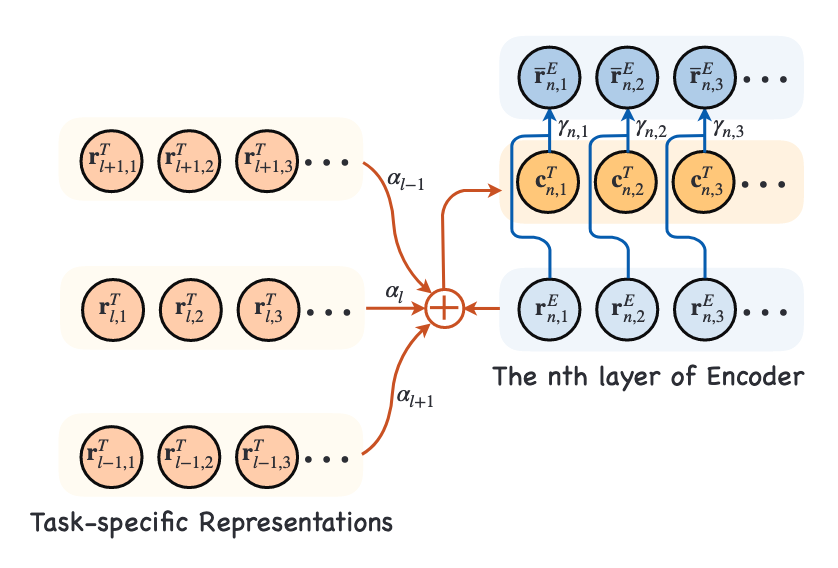
\includegraphics[width=0.95\textwidth]{img/dynamic_fusion.png}}
    \centering
    \caption{Illustration of seq2seq architecture. Figure reprinted from \cite{weng2020acquiring}.}
    \label{img:dyn_fn}
\end{figure}

\cite{yang2020towards}

compared to other tasks working well with direct BERT finetuning, NMT has two distinct characteristics, the availability of large training data (10 million or larger) and the high capacity of baseline NMT models (i.e. Transformer). These two characteristics require a huge number of updating steps during training in order to fit the high-capacity model well on massive data 1 . Updating too much leads to the catastrophic forgetting problem (Goodfellow et al. 2013), namely too much updating in training make the BERT forget its universal knowledge from pre-training. The assumption lies well with previous observations that fixed BERT improves NMT a bit and fine-tuning BERT even offers no gains. In this paper, we propose the concerted training approach (CT NMT ). Specifically, we introduce three techniques to integrate the power of pre-trained BERT and vanilla NMT, namely asymptotic distillation, dynamic switch for knowledge fusion, and ratescheduled updating. First, an asymptotic distillation (AD) technique is introduced to keep remind the NMT model of BERT knowledge. The pre-trained BERT serves as a teacher network while the encoder of the NMT model serves as a student. The objective is to mimic the original teacher network by minimizing the loss (typically L2 or cross-entropy loss) between the student and the teacher in an asymptotic way. The asymptotic distillation does not introduce additional parameters therefore it can be trained efficiently. Secondly, a dynamic switching gate (DS) is introduced to combine the encoded embedding from BERT and the encoder of NMT. Based on the source input sentence, it provides an adaptive way to fuse the power of BERT and NMT's encoder-decoder network. The intuition is that for some source sentences BERT might produce a better encoded information than NMT's encoder while it is opposite for other sentences. Thirdly, we develop a scheduling policy to adjust the learning rate during the training. Without such a technique, traditionally BERT and NMT are updated uniformly.  However, a separate and different updating pace for BERT LM is beneficial for the final combined model. Our proposed rate-scheduled learning effectively controls the separate paces of updating BERT and NMT networks according to a policy. With all these techniques combined, CT NMT empirically works effectively in machine translation tasks.

\begin{figure}[h]
    {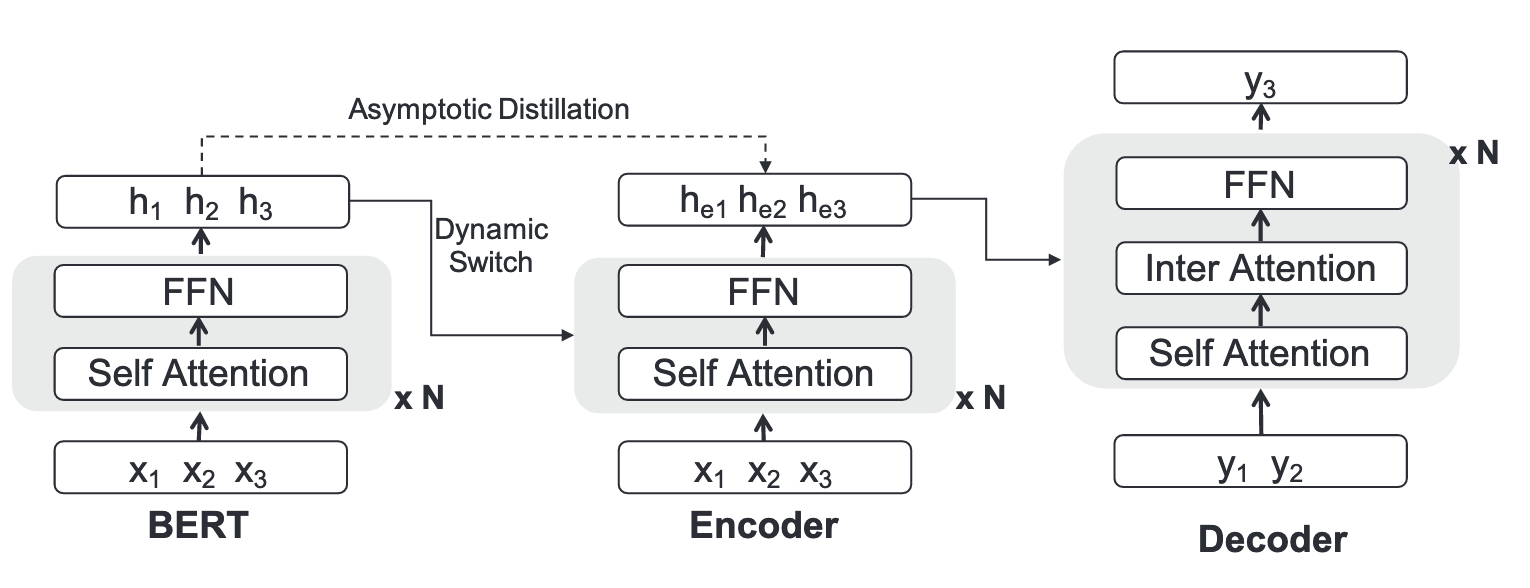
\includegraphics[width=0.95\textwidth]{img/ctnmt.png}}
    \centering
    \caption{Illustration of seq2seq architecture. Figure reprinted from \cite{yang2020towards}.}
    \label{img:ctnmt}
\end{figure}

Intuitively, as BERT is learned with a generative objective via Masked Language Modeling (MLM) during the pre-training stage, a natural assumption is that this training objective should have learned essential, bidirectional, contextual knowledge that can help enhance text generation. Unfortunately, this MLM objective is not auto-regressive, which encumbers its direct application to auto-regressive text generation in practice. In this paper, we tackle this challenge by proposing a novel and generalizable approach to distilling knowledge learned in BERT for text generation tasks. We first propose a new Conditional Masked Language Modeling (C-MLM) task, inspired by MLM but requiring additional conditional input, which enables fine-tuning pre-trained BERT on a target dataset. In order to extract knowledge from the fine-tuned BERT and apply it to a text generation model, we leverage the fine-tuned BERT as a teacher model that generates sequences of word probability logits for the training samples, and treat the text generation model as a student network, which can effectively learn from the teacher's outputs for imitation. The proposed approach improves text generation by providing a good estimation on the word probability distribution for each token in a sentence, consuming both the left and the right context, the exploitation of which encourages conventional text generation models to plan ahead. With our proposed approach, BERT's looking into the future ability can act as an effective regularization method, capturing subtle long-term dependencies that ensure global coherence and in consequence boost model performance on text generation.

\cite{chen2019distilling}

\begin{figure}[h]
    {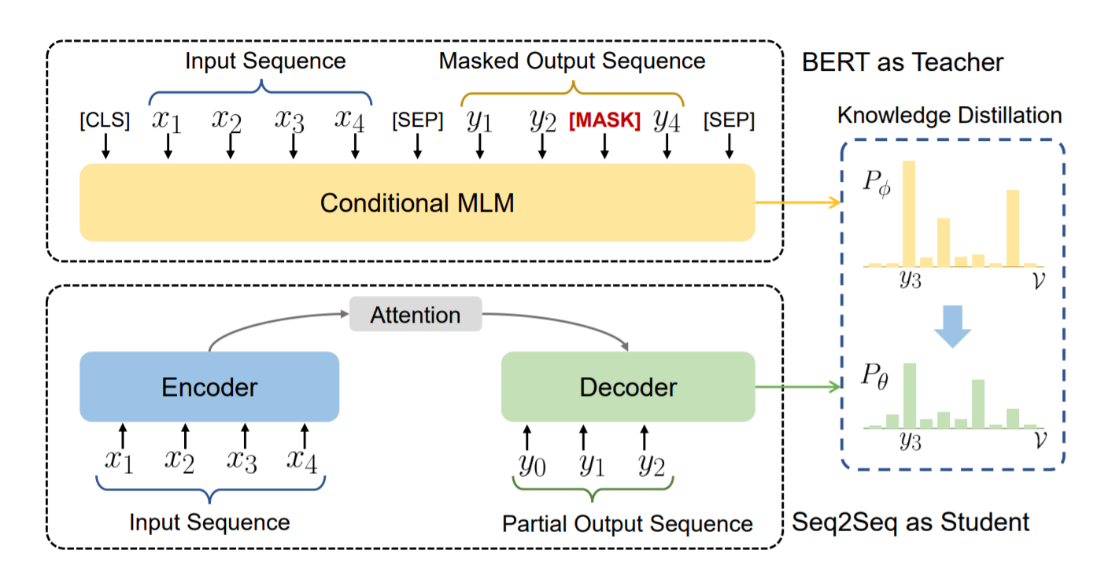
\includegraphics[width=0.95\textwidth]{img/bert_distill.png}}
    \centering
    \caption{Illustration of seq2seq architecture. Figure reprinted from \cite{chen2019distilling}.}
    \label{img:bert_distill}
\end{figure}

\section{Adapters in Sequence-to-Sequence}
\label{sec:adapter_seq}

In this section, we divide the discussion and reviews in three sections. The first Section \ref{sec:adapter_place} discuss the importance of adapters placement in the transformer layers as well as in the sequence to sequence framework. The first part reviews the work of \cite{houlsby2019parameter} and \cite{bapna2019simple}. Both works propose the same concept of adapters with similar architecture. The difference between them lies in the placement of the adapters within the transformer layer. The other work by \cite{winata2020adapt} discuss the importance of adapters in sequence to sequence framework. They found interesting result where adapters in one component has more impact than in the other component.

Section \ref{sec:app_nlu_asr} and \ref{sec:app_mt} will each review the application of adapters in other fields such as NLU and ASR as well as in the machine translation. Each discussion will contain the type of adapters that used, the purpose of the adapters, and the impact of including the adapters as a part of their training procedure.

\subsection{Placement of Adapters}
\label{sec:adapter_place}
As of this writing, there are two types of adapters placement in the transformer architecture. The adapters on the first work by \cite{houlsby2019parameter}, is always applied directly to the output of the sub-layer, after the projection back to the input size, but before adding the skip connection back. The output of the adapter is then passed directly into the following layer normalization. Each layer of the Transformer contains two primary sub-layers: an attention layer and a feedforward layer. Both layers are followed immediately by a projection that maps the features size back to the size of layer's input. A skip-connection is applied across each of the sub-layers. The output of each sub-layer is fed into layer normalization. They insert two serial adapters after each of these sub-layers. The adapter is always applied directly to the output of the
Types of adapters (at the end of network and in sub-network). The illustration of the adapter architecture can be seen at Figure \ref{img:ada_houlsby}.

\begin{figure}[h]
    {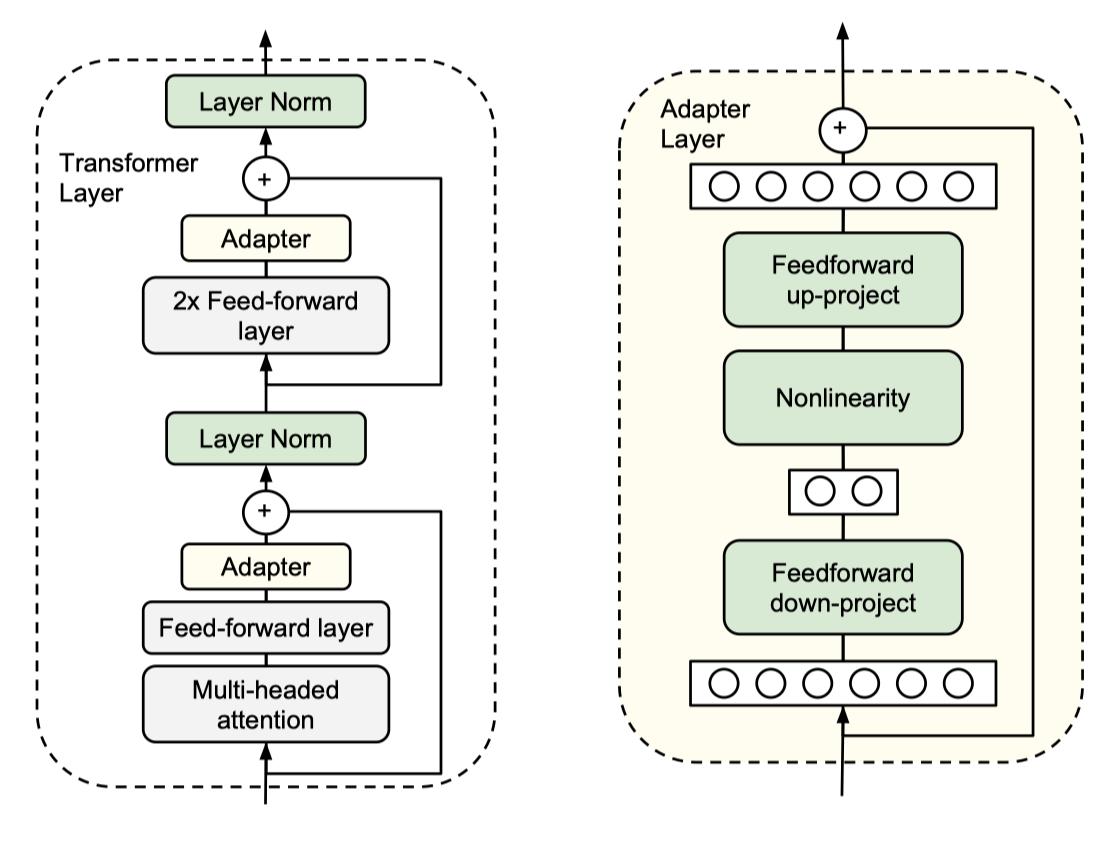
\includegraphics[width=0.95\textwidth]{img/adapter_houlsby.png}}
    \centering
    \caption{Illustration of adapter architecture. Figure reprinted from \cite{houlsby2019parameter}.}
    \label{img:ada_houlsby}
\end{figure}

The second work of adapters is published by \cite{bapna2019simple}. They took a simpler approach in contrast to \cite{houlsby2019parameter} in regards of incorporating the adapters into the transformer network. Rather than inserting two serial adapters into the sub-layers of transformer, they just instantiate a single instance of adapters and place it on the top of each layers. In addition to the simpler design of adapter layers, they add layer normalization to normalize the input of the adapters. The reasoning behind this is to make the adapters plug-able into any part of the base networks, ignoring the distribution variations of the previous layers. For illustration we refer to Figure \ref{img:ada_bapna}

\begin{figure}[h]
    {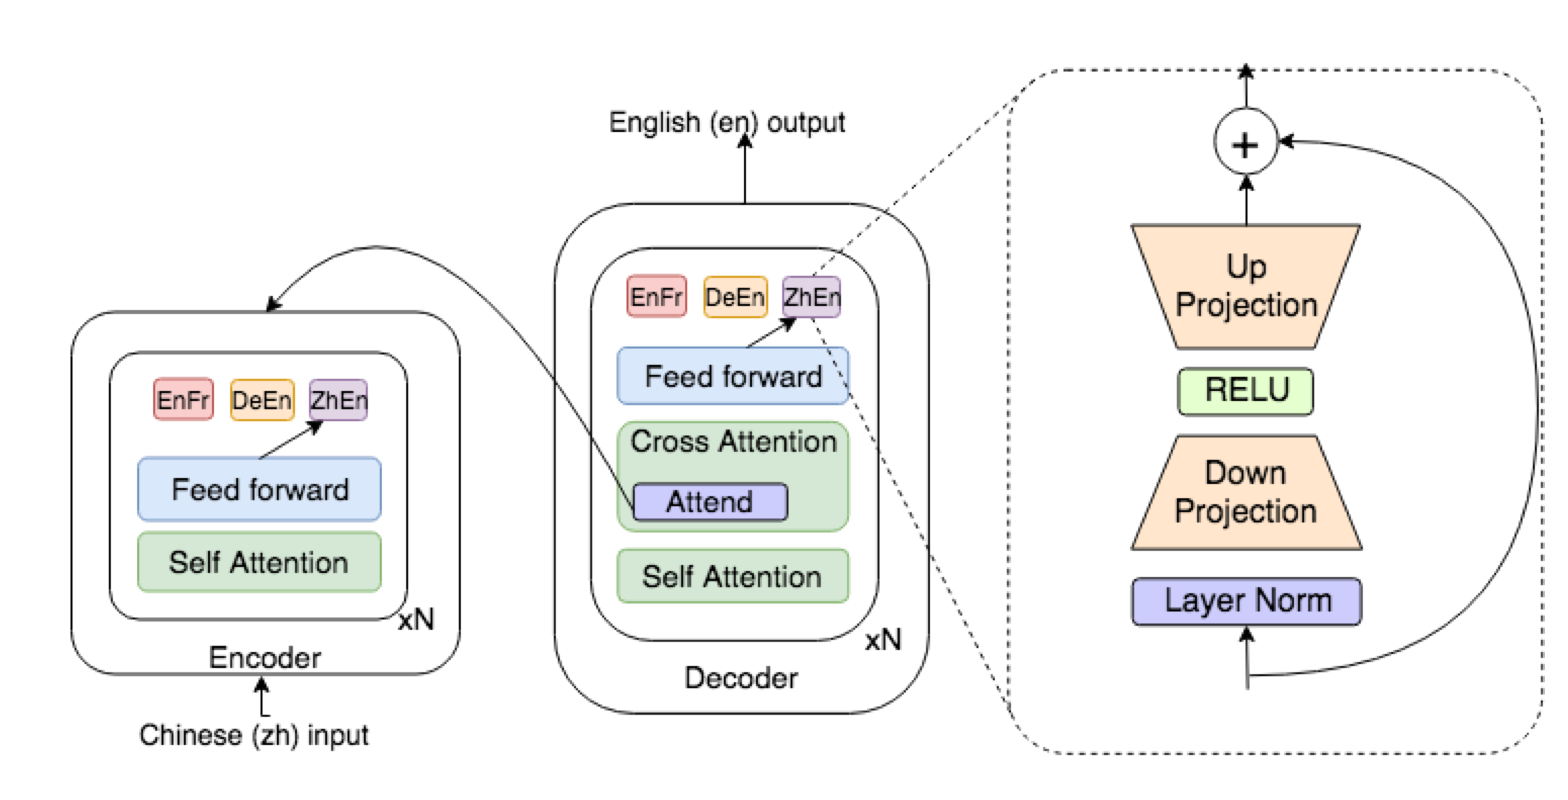
\includegraphics[width=0.95\textwidth]{img/adapter_bapna.png}}
    \centering
    \caption{Illustration of adapter architecture. Figure reprinted from \cite{bapna2019simple}.}
    \label{img:ada_bapna}
\end{figure}

\cite{pfeiffer2021adapterfusion} mentioned that the placement of adapter parameters within a pretrained model is non-trivial, and thus requires extensive experiments. To identify the best setup for the adapters placement, the authors perform an exhaustive search on the hyperparameters. This include the position and the number of adapters within a single layer, the position of residual connections, th bottleneck residual factors, as well as the non-linearity within the bottleneck adapter layer. In their experiments that involve both NLU and NLG, they find the best performing adapter is close to the simple architecture proposed by \cite{bapna2019simple} and not from \cite{houlsby2019parameter}.

We now discuss the placement of the adapters from the perspective of encoder-decoder framework (seq2seq). \cite{winata2020adapt} conducted an experiment using similar adapter architecture and placement to \cite{bapna2019simple} in ASR task. The encoder in this work represents a model whose job is to encode audio representation. On the other hand, the decoder is responsible to encode the text features as well as generate text output. In this work, the authors perform experiments comparing the effectiveness of adapters in both encoder and decoder. They initialized the decoder using pre-trained mBERT weights (\cite{devlin2018bert}). Based on their findings, adapters in decoder are not as effective as they are in the encoder component. This results indicate that adapting the weights in audio space is more effective to the model's performance than in the text space. This is probable that features in mBERT has already provided enough good features so that further fine-tuning may no longer be necessary.

\subsection{Adapters in NLU and Automatic Speech Recognition}
\label{sec:app_nlu_asr}
As of this writing, adapters has been used as an alternative for naive fine-tuning in various fields in NLP. \cite{houlsby2019parameter} introduces adapters to fine-tune BERT model in various NLU tasks. Primarily, they test the adapters in GLUE \cite{wang2018glue} and additional classification tasks. They further their experiments in a more complicated problem such as SQuAD \cite{rajpurkar2018know}. We can refer to Section \ref{sec:adapter_place} for the explanation and illustration of the adapters architecture of their work. They found positive results of using adapters in GLUE, additional classification, and SQuAD tasks compared to the fine-tuning. By adding a small number of parameters, they achieved a comparable performance in all tasks compared to fine-tuning the whole weights.

\cite{pfeiffer2020madx} works in adapters involve bootstrapping pre-trained NLP models such as BERT, and XLM \cite{conneau2019cross} in low-resource languages. They perform two types of adaptation, language-adaptation and task-adaptation. For this purpose, they use two different adapters used in different situations. The language-adapters are trained in MLM objective to capture various features in different languages. They then put task-adapters on top of the language adapters for further fine-tuning for each of the tasks in their experiments. They use an efficient adapters architecture based on \cite{pfeiffer2021adapterfusion} works which have similarity to the work in \cite{bapna2019simple}. For more details on the architecture definition, we refer the reader to Section \label{sec:bm_adapters}. They perform their experiments on three different tasks: Named Entity Recognition (NER), extractive question answering (QA), and causal commonsense reasoning (CCR). Each of these tasks is available in multi-languages that include high-resource and low-resource languages. We suggest the reader to their original paper for more details on the dataset they used on each of the tasks. Their main finding is that the task-specific adapters perform similar to the work in \cite{houlsby2019parameter}. However, since their main focus is on multilingual setup, they did not find satisfying results due to discrepancies in unseen languages. With the help of language-adapters, they managed to bridge the missing gap and have improved performance across all tasks. The performance is especially appealing in low-resource languages.

\cite{winata2020adapt} evaluates adapters performance in multilingual ASR setup. They use a similar setup as \cite{bapna2019simple} to adapt both the encoder and decoder. They employ adapters to combat language mismatch and improve models' robustness in various languages with limited resources. Their main finding for the adapters is that it improves the performance across various languages. Furthermore, they also performed experiments to generate a cluster of languages where similar languages are put within the same group. They then share the adapters to languages belonging to the same group and find out that this helps performance in low-resource languages but has small drawbacks in the high resource languages.

\cite{lee2021adaptable} propose a multi-domain adapters for language model in ASR setup. Specifically, they employ the adapters to adapt the language model (LM) component for rescoring purposes in an ASR system. They use the similar architecture of the adapter to the work of \cite{houlsby2019parameter} where they introduce adapters within the sub-networks as well as the top of the layer. Their experiments show that by using separate adapters for each domain, they can easily re-use a general domain LM and switching domain by replacing adapters to the one that has already been fine-tuned on the respective domain. They also found that with the help of adapters, they manage to improve the performance on a specific problem, such as predicting proper nouns.

\subsection{Adapters in Machine Translation}
\label{sec:app_mt}
\cite{bapna2019simple} propose an alternative from \cite{houlsby2019parameter} where instead of using two different adapters in a single transformer layer, they propose to just use a single adapters on top of the layer. Another difference is that they add a layer normalization after the transformer layer output. Furthermore, they also experiment with the adaptesr in NLG domain instead of NLU> In this work, they use machine translation objective and treat the adapters as the adaptation module for a certain language pair. They first pre-trained the model in a large corpus such as WMT before they perform domain adaptation to a smaller corpus such as IWSLT in the same language pair. On a single language pair experiment, they found out that the proposed adapters architecture is flexible to the size of the data by adjusting the adapter's capacity to match the requirements for the corpus size adaptation. Furthermore, they found out that by having a reasonably small adapter size, they did not found a sign of overfitting and instead they found the model to reach its peak and stays steady throughout the training process.

\cite{philip2020monolingual} applies adapters in multilingual machine translation in different way than \cite{bapna2019simple}. \cite{bapna2019simple} uses adapters for every target pairs. For example, in English France pair, they have to create two different adapters for English$\rightarrow$France and France$\rightarrow$English. \cite{philip2020monolingual} propose to use monolingual adapter where instead of using a single adapter for a language pair, they use a single adapter for each of the languages. They use the same adapter architecture as in \cite{bapna2019simple} to perform the experiments. Their findings suggest that their approach managed to reduce the number of adapters from $n(n-1)$ to $2n$. Furthermore, they also find that this approach have better performance in low-resource languages than the one proposed in \cite{bapna2019simple}.

\cite{guo2021adaptive} shows that adding adapters to BERT during the fine-tuning can be beneficial in machine translation task. The purpose of the adapters in this work is to replace the regular fine-tuning mechanism so that the training process is more lightweight. They follow the adapters architecture and similar mechanism to include the adapters on the base model from \cite{bapna2019simple}. The difference is that in \cite{bapna2019simple} they do not use BERT as the base model and use plain transformer that pre-trained using machine translation objective. Although BERT itself is still using transformer, they already contain information from the previous pre-training.
% The difficulties of incorporating BERT in machine translation has already explained in \ref{sec:domain_adapt}. \cite{guo2021adaptive} also propose that


% \section{Fine-tuning in Sequence-to-Sequence Framework}